\section{Lenguajes regulares}

\subsection{Palabras y autómatas}

\subsubsection{Palabras}

\paragraph{Definiciones.} Consideremos que:

\begin{itemize}
    \item Un \textbf{alfabeto} $\Sigma$ es con conjunto finito.
    \item Un elemento de $\Sigma$ lo llamaremos una \textbf{letra} o \textbf{símbolo}.
    \item Una \textbf{palabra} o \textbf{string} sobre $\Sigma$ es una secuencia finita de letras en $\Sigma$.
          \ejemplo{}{}{
              \begin{itemize}
                  \item $\Sigma = \{a,b,c\}$
                  \item Palabras sobre $\Sigma$:
                        $$
                            aaaaabb,\ bcaabab, \ a,\ bbbbbb,\ \cdots
                        $$
              \end{itemize}
          }
    \item El largo $|w|$ de una palabra $w$ es el número de letras.
          \alignformula{
              |w| \overunder{\equiv}{}{\text{def}} \# \text{ de letras en } w
          }
    \item Denotaremos $\epsilon$ como la \textbf{palabra sin símbolos} de largo $0$.
          \alignformula{
              |\epsilon| \overunder{\equiv}{}{\text{def}} 0
          }
    \item Denotaremos por $\Sigma^*$ como el \textbf{conjunto de todas las palabras} sobre $\Sigma$.
          \ejemplo{}{}{
              Para $\Sigma = \{0,1\}$:
              \begin{itemize}
                  \item $|00011001| = 8$
                  \item $\Sigma^* =$ todas las palabras posibles formadas por 0s y 1s.
              \end{itemize}
          }
\end{itemize}

\paragraph{Definición.} Dados dos palabras $u,v \in \Sigma^*$ tal que $u = a_1 \ldots a_n$ y $v = b_1 \ldots v_m$:
\alignformula{
    u \cdot v \overunder{\equiv}{}{\text{def}} a_1 \ldots a_n b_1 \cdots b_m
}
Decimos que $u \cdot v$ es la palabra ``$u$ \textbf{concatenada} con $v$''.
\ejemplo{}{}{
    Para $\Sigma = \{0,1,2,\ldots,9\}$:
    \begin{itemize}
        \item $0123\cdot 9938 = 01239938$ y $3493 \cdot \epsilon = 3493$
    \end{itemize}
}

\paragraph{Propiedades de concatenación.} La concatenación cumple:
\begin{itemize}
    \item \textbf{Asociatividad:} $(u \cdot v) \cdot w = u \cdot (v \cdot w)$
    \item \textbf{Largo:} $|u\cdot v| = |u| + |v|$
    \item ¿Cumple conmutatividad? No. Por ejemplo, si $u = ab$ y $v = bb$, entonces $u \cdot v = abbb \neq bbab = v \cdot u$.
\end{itemize}

\paragraph{Definición.} Sea $\Sigma$ un alfabeto y $L \subseteq \Sigma^*$. Decimos que $L$ es un \textbf{lenguaje} sobre el alfabeto $\Sigma$.
\ejemplo{}{}{
    Sea $\Sigma = \{a,b\}$:
    \begin{itemize}
        \item $L_0 = \{\epsilon, a, aa, b, aa\}$
        \item $L_1 = \{\epsilon, b, bb, bbb, bbbb, \ldots\}$
        \item $L_2 = \{w \,|\, \exists u \in L_1, w = a \cdot u\}$
        \item $L_3 = \{w \,|\, \exists u,v \in \Sigma^*, w = u \cdot abba \cdot v\}$
        \item $L_4 = \{w \,|\, \exists u \in \Sigma^*,w = u \cdot u\}$
    \end{itemize}
}
Un \textbf{lenguaje} puede ser visto como una \textbf{propiedad} de palabras.

\paragraph{Convenciones.} Durante todo este texto:
\begin{itemize}
    \item Para \textbf{letras} se usarán los símbolos: $a,b,c,d,e,\ldots$
    \item Para \textbf{palabras} se usarán los símbolos: $w,u,v,x,y,z,\ldots$
    \item Para \textbf{alfabetos} se usarán los símbolos: $\Sigma,\Gamma,\ldots$
    \item Para \textbf{lenguajes} se usarán los símbolos: $L,M,N,\ldots$
    \item Para \textbf{números} se usarán los símbolos: $i,j,k,l,m,n,\ldots$
\end{itemize}

\subsubsection{Autómatas}
Una autómata \textbf{finito} es:
\begin{itemize}
    \item Un modelo de computación sencillo, basado en una cantidad \textbf{finita} de memoria.
    \item Procesa cada \textbf{palabra} de principio a fin en \textbf{una sola pasada}.
    \item Al terminar, el autómata decide si \textbf{acepta} o \textbf{rechaza} el input.
\end{itemize}
Usaremos los autómatas finitos para definir \textbf{lenguajes}.

\paragraph{Definición.} Un autómata finito determinista (DFA) es una tupla:
\alignformula{
    \ca{A} = (Q,\Sigma,\delta,q_0,F)
}
\begin{multicols}{2}
    \begin{itemize}
        \item $Q$ es un conjunto finito de \textbf{estados}.
        \item $\Sigma$ es el alfabeto del \textbf{input}.
        \item $\delta: Q \times \Sigma\rightarrow Q$  es la función de \textbf{transición}.
        \item $q_0 \in Q$ es el \textbf{estado inicial}.
        \item $F \subseteq Q$ es el conjunto de \textbf{estados finales} (o aceptación).
    \end{itemize}
\end{multicols}

\ejemplo{}{}{
    \begin{itemize}
        \item $Q = \{0,1,2\}$
        \item $\Sigma = \{a,b\}$
        \item $\delta:Q \times \Sigma \to Q$ se define como:
              $$
                  \begin{aligned}
                      \delta(0, a) & =1                              \\
                      \delta(1, a) & =2                              \\
                      \delta(2, a) & =2                              \\
                      \delta(q, b) & =q \quad \forall q \in\{0,1,2\}
                  \end{aligned}
              $$
        \item $q_0 = 0$
        \item $F= \{2\}$
    \end{itemize}
    \img{img/cap1/ejemplo5.png}{0.45}
}

\paragraph{Ejecución.} Sea $\ca{A}=(Q,\Sigma,\delta,q_0,F)$ un DFA y $w = a_1 a_2 \ldots a_n \in \Sigma^*$ un input. Una \textbf{ejecución} (o \textit{run}) $\rho$ de $\ca{A}$ sobre $w$ es una secuencia:
\alignformula{
    \rho: \quad p_0 \stackrel{a_1}{\rightarrow} p_1 \stackrel{a_2}{\rightarrow} p_2 \stackrel{a_3}{\rightarrow} \ldots \stackrel{a_n}{\rightarrow} p_n
}
donde $p_0 = q_0$ y para todo $i \in \{0,1,\ldots,n-1\}$ se cumple que $\delta(p_i,a_{i+1}) = p_{i+1}$. \medbreak

Una ejecución $\rho$ de $\ca{A}$ sobre $w$ es de \textbf{aceptación} si $p_n \in F$.

\ejemplo{}{}{
    \img{img/cap1/ejemplo5.png}{0.45}
    \begin{itemize}
        \item ¿Cuál es la ejecución de $\ca{A}$ sobre $bbab$? \medbreak

              $\rho: 0 \overset{b}{\rightarrow} 0 \overset{b}{\rightarrow} 0 \overset{a}{\rightarrow} 1 \overset{b}{\rightarrow} 1$. La ejecución \textbf{no} es de aceptación ya que no termina en un estado final.

        \item ¿Cuál es la ejecución de $\ca{A}$ sobre $abab$? \medbreak

              $\rho: 0 \overset{a}{\rightarrow} 1 \overset{b}{\rightarrow} 1 \overset{a}{\rightarrow} 2 \overset{b}{\rightarrow} 2$. La ejecución \textbf{si} es de aceptación ya que termina en un estado final.
    \end{itemize}
}

\paragraph{Aceptación.} Sea $\ca{A} = (Q,\Sigma,\delta,q_0,F)$ un DFA y $w \in \Sigma^*$. Decimos que $\ca{A}$ \textbf{acepta} $w$ si la ejecución de $\ca{A}$ sobre $w$ es de aceptación. Al contrario, decimos que $\ca{A}$ \textbf{rechaza} $w$ si la ejecución de $\ca{A}$ sobre $w$ NO es de aceptación. \medbreak

El \textbf{lenguaje aceptado} por $\ca{A}$ se define como:
\alignformula{
    \ca{L}(\ca{A}) = \{w \in \Sigma^* \mid \ca{A} \text{ acepta } w\}
}

Un lenguaje $L \subseteq \Sigma^*$ se dice \textbf{regular} si, y sólo si, \textbf{existe} un autómata finito determinista $\ca{A}$ tal que
\alignformula{
    L = \ca{L}(\ca{A})
}

\subsection{Construcciones de autómatas}

Veremos una definición alternativa al autómata visto en la sección anterior.

\subsubsection{Autómatas con función parcial de transición}

\paragraph{Definición.} Un autómata finito determinista con \textbf{función parcial de transición} (DFAp) es una tupla:

\alignformula{
    \ca{A} = (Q, \Sigma, \gamma, q_0, F)
}
\begin{itemize}

    \item $Q$ es un conjunto finito de estados.
    \item $\Sigma$ es el alfabeto del input.
    \item $\gamma: Q \times \Sigma\rightharpoonup Q$  es una \textbf{función parcial de transición}.
    \item $q_0 \in Q$ es el estado inicial.
    \item $F \subseteq Q$ es el conjunto de estados finales (o aceptación).
\end{itemize}

\paragraph{Ejecución.} Sea $w = a_1 a_2 \ldots a_n \in \Sigma^*$. De igual manera que un DFA, una \textbf{ejecución} (o \textit{run}) $\rho$ de $\ca{A}$ sobre $w$ es una secuencia:
\alignformula{
    \rho: p_0 \stackrel{a_1}{\rightarrow} p_1 \stackrel{a_2}{\rightarrow} p_2 \ldots \stackrel{a_n}{\rightarrow} p_n
}
donde $p_0 = q_0$ y para todo $i \in \{0,\ldots,n-1\}$ \textbf{está definido} $\gamma(p_i, a_{i+1}) = p_{i+1}$. \medbreak

Una ejecución $\rho$ de $\ca{A}$ sobre $w$ es de \textbf{aceptación} si $p_n \in F$. Notemos que ahora una palabra puede NO tener una ejecución.

\paragraph{Aceptación.} Sea $\ca{A}$ un DFAp y $w \in \Sigma^*$. Decimos que $\ca{A}$ \textbf{acepta} $w$ si \textbf{existe una ejecución} de $\ca{A}$ sobre $w$ que es de aceptación. También, el \textbf{lenguaje aceptado} por $\ca{A}$ se define como:

\alignformula{
    \ca{L}(\ca{A}) = \{ w \in \Sigma^* \mid \ca{A} \text{ acepta } w \}
}

\ejemplo{}{}{
    \begin{figure}[H]
        \centering
        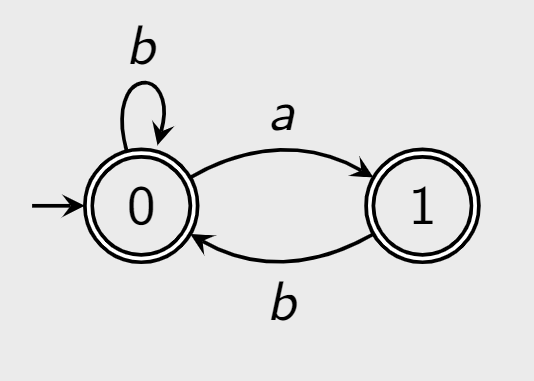
\includegraphics[scale=0.3]{img/cap1/ejemplo7_1.png}
        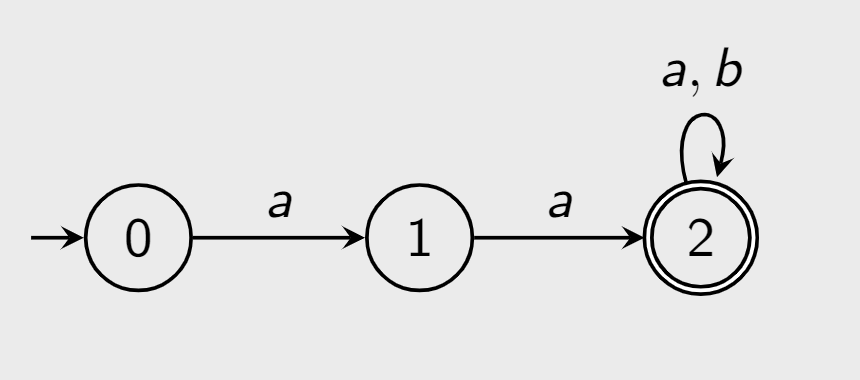
\includegraphics[scale=0.3]{img/cap1/ejemplo7_2.png}
    \end{figure}
}

\paragraph{¿DFA $\not\equiv$ DFAp?} Establezcamos una proposición. Para todo autómata $\ca{A}$ con función parcial de transición, existe un autómata $\ca{A}'$ (con función total de transición) tal que:
\alignformula{
    \ca{L}(\ca{A}) = \ca{L}(\ca{A}')
}
En otras palabras, DFA $\equiv$ DFAp.

\paragraph{Demostración.} Sea $\ca{A} = (Q,\Sigma,\gamma,q_0,F)$ un autómata con función parcial de transición. Sea $q_s$ un \textbf{nuevo estado} tal que $q_s \notin Q$. Contruimos el DFA $\ca{A}' = (Q \cup \{q_s\}, \Sigma, \delta', q_0, F)$ tal que:
$$
    \delta^{\prime}(p, a)= \begin{cases}\gamma(p, a) & \text { si } p \neq q_s \text{ y }(p, a) \in \operatorname{dom}(\gamma) \\ q_s & \text { si no }\end{cases}
$$
para todo $p \in Q \cup \{q_s\}$ y $a \in \Sigma$. Queremos demostrar que $\ca{L}(\ca{A}) = \ca{L}(\ca{A}')$.

\paragraph{Dem. $\ca{L}(\ca{A}) \subseteq \ca{L}(\ca{A}')$.} Sea $w = a_1\ldots a_n \in \ca{L}(\ca{A})$. Entonces, existe una ejecución de aceptación $\rho$ de $\ca{A}$ sobre $w$:
$$
    \rho: p_0 \stackrel{a_1}{\rightarrow} p_1 \stackrel{a_2}{\rightarrow} p_2 \ldots \overset{a_n}{\rightarrow} p_n
$$
donde $p_0 = q_0$, para todo $i \in \{0,\ldots,n-1\}$ está definido $\gamma(p_i,a_{i+1}) = p_{i+1}$ y $p_n \in F$. Como $\delta'(p_i, a_{i+1}) = \gamma(p_i,a_{i+1})$ para todo $i \in \{0,\ldots,n-1\}$ (por la definición de $\delta'$), entonces $\rho$ es también una ejecución de aceptación de $\ca{A}'$ sobre $w$. Por lo tanto, $w \in \ca{L}(\ca{A}')$.

\paragraph{Dem. $\ca{L}(\ca{A}') \subseteq \ca{L}(\ca{A})$.} Sea $w = a_1\ldots a_n \in \ca{L}(\ca{A}')$. Entonces, existe una ejecución de aceptación $\rho$ de $\ca{A}'$ sobre $w$:
$$
    \rho: p_0 \stackrel{a_1}{\rightarrow} p_1 \stackrel{a_2}{\rightarrow} p_2 \ldots \overset{a_n}{\rightarrow} p_n
$$
donde $p_0 = q_0$, para todo $i \in \{0,\ldots,n-1\}$ tenemos $\gamma'(p_i,a_{i+1}) = p_{i+1}$ y $p_n \in F$. Demostraremos que $p_i \neq q_s$ para todo $i \in \{0,\ldots, n\}$. Por \textbf{contradicción}, suponga que existe $i$ tal que $p_i = q_s$. entonces, tenemos que $p_{i+1} = q_s$. Por \textbf{inducción}, podemos demostrar que $p_j = q_s$ para todo $j \ge i$, y así, podemos concluir que $p_n = q_s$, llevándonos a una contradicción. Como $p_i \neq q_s$ para todo $i \in \{0, \ldots, n\}$, tenemos que:
$$
    \delta^{\prime}\left(p_i, a_{i+1}\right)=\gamma\left(p_i, a_{i+1}\right) \quad \forall i \in\{0,1, \ldots, n-1\}
$$
y entonces $\rho$ es una \textbf{ejecución de aceptación} de $\ca{A}$ sobre $w$. Por lo tanto, concluimos que $w \in \ca{L}(\ca{A})$. \hfill $\blacksquare$

\paragraph{Advertencia.} Desde ahora, se utilizaran autómatas con funciones \textbf{totales} de transición, pero sin pérdida de generalidad, en algunos ejemplos habrán autómatas con funciones \textbf{parciales} de transición por simplicidad.

\subsubsection{Operaciones de conjuntos}
\paragraph{Definiciones.} Dado dos lenguajes $L,L' \subseteq \Sigma^*$ se define:
\alignformula{
    \begin{aligned}
        L^C               & =\left\{w \in \Sigma^* \mid w \notin L\right\}                      \\
        L \cap L^{\prime} & =\left\{w \in \Sigma^* \mid w \in L \wedge w \in L^{\prime}\right\} \\
        L \cup L^{\prime} & =\left\{w \in \Sigma^* \mid w \in L \vee w \in L^{\prime}\right\}
    \end{aligned}
}

Dado dos autómatas $\ca{A}$ y $\ca{A}'$:
\begin{enumerate}
    \item ¿Existe un autómata $\ca{B}$ tal que $\ca{L}(\ca{B}) = \ca{L}(\ca{A})^C$?
    \item ¿Existe un autómata $\ca{B}$ tal que $\ca{L}(\ca{B}) = \ca{L}(\ca{A}) \cap \ca{L}(\ca{A}')$?
    \item ¿Existe un autómata $\ca{B}$ tal que $\ca{L}(\ca{B}) = \ca{L}(\ca{A}) \cup \ca{L}(\ca{A}')$?
\end{enumerate}

\paragraph{Construcción de $\ca{L}(\ca{A})^C$.} Dado un autómata $\ca{A} = (Q, \Sigma, \delta, q_0, F)$, definimos el autómata:
\alignformula{
    \mathcal{A}^C=\left(Q, \Sigma, \delta, q_0, Q \backslash F\right)
}
\teorema{}{}{
    Para todo autómata $\ca{A}$, se tiene que $\ca{L}(\ca{A})^C = \ca{L}(\ca{A}^C)$.
}

\paragraph{Producto de autómatas.} Suponga que:
$$
    \begin{aligned}
        \mathcal{A}          & =\left(Q, \Sigma, \delta, q_0, F\right)                                     \\
        \mathcal{A}^{\prime} & =\left(Q^{\prime}, \Sigma, \delta^{\prime}, q_0^{\prime}, F^{\prime}\right)
    \end{aligned}
$$
y considere una palabra $w \in \Sigma^*$. ¿Cómo ejecutamos ambos autómatas sobre $w$ al \textbf{mismo tiempo}? La idea es ejecutar $\ca{A}$ y $\ca{A}'$ \textbf{en paralelo}. Así, definimos el \textbf{producto} entre $\ca{A}$ y $\ca{A}'$ como el autómata $\ca{A} \times \ca{A}' = (Q^\times, \Sigma, \delta^\times, q_0^\times, F^\times)$ tal que:
\begin{itemize}
    \item $Q^\times = Q \times Q'=\{(q,q')\;|\;q\in Q \wedge q' \in Q'\}$
    \item $\delta^\times((q,q'),a)=(\delta(q,a),\delta'(q',a))$
    \item $q^\times_0=(q_0,q'_0)$
    \item $F^\times=F\times F'$
\end{itemize}

\ejemplo{}{}{
    Todas las palabras sobre $\{a,b\}$ con una cantidad par de $a$-letras tal que no hay dos $a$-letras seguidas.
    \img{img/cap1/ejemplo8.png}{0.4}
}

\teorema{}{}{
    Para todo par de autómatas $\ca{A}$ y $\ca{A}'$ se tiene que
    $$
        \ca{L}(\ca{A} \times \ca{A}') = \ca{L}(\ca{A}) \cap \ca{L}(\ca{A}')
    $$
}

\paragraph{Demostración teorema 2.} Solo se demostrará que $\ca{L}(\ca{A}) \cap \ca{L}(\ca{A}') \subseteq \ca{L}(\ca{A} \times \ca{A}')$, la otra dirección queda propuesta para el lector. \medbreak

Sea $w = a_1 \ldots a_n \in \ca{L}(\ca{A}) \cap \ca{L}(\ca{A}')$. Entonces $w \in \ca{L}(\ca{A})$ y $w \in \ca{L}(\ca{A}')$. Existen ejecuciones de aceptación $\rho$ y $\rho'$ de $\ca{A}$ y $\ca{A}'$ sobre $w$, respectivamente:
$$
    \rho: p_0 \stackrel{a_1}{\rightarrow} p_1 \stackrel{a_2}{\rightarrow} \ldots \stackrel{a_n}{\rightarrow} p_n \quad \rho^{\prime}: p_0^{\prime} \stackrel{a_1}{\rightarrow} p_1^{\prime} \stackrel{a_2}{\rightarrow} \ldots \stackrel{a_n}{\rightarrow} p_n^{\prime}
$$
\begin{itemize}
    \item $p_0 = q_0$ y $p_0' = q_0'$.
    \item $\delta(p_{i-1},a_i) = p_i$ y $\delta'(p_{i-1}',a_i) = p_i$ para todo $i \in \{1,\ldots, n\}$.
    \item $p_n \in F$ y $p_n' \in F'$.
\end{itemize}

Por definición, tenemos que: $\rho^{\times}:\left(p_0, p_0^{\prime}\right) \stackrel{a_1}{\rightarrow}\left(p_1, p_1^{\prime}\right) \stackrel{a_2}{\rightarrow} \ldots \stackrel{a_n}{\rightarrow}\left(p_n, p_n^{\prime}\right)$
\begin{itemize}
    \item $(p_0,p_0') = (q_0,q_0')$.
    \item $\left(p_i, p_i^{\prime}\right)=\left(\delta\left(p_{i-1}, a_i\right), \delta^{\prime}\left(p_{i-1}^{\prime}, a_i\right)\right)=\delta^{\times}\left(\left(p_{i-1}, p_{i-1}^{\prime}\right), a_i\right) \forall i \in\{1, \ldots, n\}$.
    \item $(p_n,p_n') \in F \times F'$.
\end{itemize}

Por lo tanto, $\rho^\times$ es una ejecución de $\ca{A} \times \ca{A}'$ sobre $w$ y $w \in \ca{L}(\ca{A} \times \ca{A}')$. \hfill $\blacksquare$

\paragraph{Unión de autómatas.} Sabemos que
$$
    \mathcal{L}(\mathcal{A}) \cup \mathcal{L}\left(\mathcal{A}^{\prime}\right)=\left(\mathcal{L}(\mathcal{A})^C \cap \mathcal{L}\left(\mathcal{A}^{\prime}\right)^C\right)^C
$$

Para calcular el autómata que acepta el lenguaje $\ca{L}(\ca{A}) \cup \ca{L}(\ca{A}')$:
\begin{enumerate}
    \item Complementamos $\ca{A}$ y $\ca{A}'$.
    \item Intersectamos $\ca{A}^C$ y $(\ca{A}')^C$.
    \item Complementamos $\ca{A}^C \times (\ca{A}')^C$.
\end{enumerate}

\subsection{No-determinismo}

\textit{``Indeterminism is the concept that events (certain events, or events of certain types) are not caused deterministically (cf.  causality) by prior events. It is the opposite of \textbf{determinism} and related to chance. It is highly relevant to the philosophical problem of \textbf{free will}.''} - Wikipedia.

\subsubsection{Definición de un NFA}

\paragraph{Definición.} Un autómata finito \textbf{no-determinista} (NFA) es una estructura:
\alignformula{
    \ca{A} = (Q,\Sigma, \Delta, I, F)
}
\begin{itemize}
    \item $Q$ es un conjunto finito de estados.
    \item $\Sigma$ es el alfabeto del input.
    \item $F \subseteq Q$ es el conjunto de estados finales (o aceptación).
    \item $\Delta \subseteq Q \times \Sigma \times Q$ es la \textbf{relación de transición}.
    \item $I \subseteq Q$ es un \textbf{conjunto de estados iniciales}.
\end{itemize}

\ejemplo{}{}{
    \begin{itemize}
        \item $Q = \{0,1,2\}$, $\Sigma = \{a,b\}$, $I = \{0,1\}$, $F = \{2\}$
        \item $\Delta \subseteq Q \times \Sigma \times Q$ se define como:
              \img{img/cap1/ejemplo9.png}{0.4}
    \end{itemize}
}

\paragraph{Ejecución.} Sea $\ca{A} = (Q,\Sigma,\Delta, I, F)$ un NFA y $w = a_1 a_2 \ldots a_n \in \Sigma^*$ el input. Una \textbf{ejecución} (o \textit{run}) $\rho$ de $\ca{A}$ sobre $w$ es una secuencia:
\alignformula{
    \rho: p_0 \stackrel{a_1}{\rightarrow} p_1 \stackrel{a_2}{\rightarrow} \ldots \stackrel{a_n}{\rightarrow} p_n
}
donde $p_0 \in I$ y para todo $i \in \{0,\ldots,n-1\}$, se tiene que $(p_i, a_{i+1}, p_{i+1}) \in \Delta$. \medbreak

Una ejecución $\rho$ de $\ca{A}$ sobre $w$ es de \textbf{aceptación} si $p_n \in F$.

\paragraph{Aceptación.} Decimos que $\ca{A}$ \textbf{acepta} $w$ si \textbf{existe} una ejecución de $\ca{A}$ sobre $w$ que es de aceptación. Por otro lado, decimos que $\ca{A}$ \textbf{rechaza} si \textbf{todas} las ejecuciones de $\ca{A}$ sobre $w$ NO son de aceptación. Además, el \textbf{lenguaje aceptado} por $\ca{A}$ se define como:
\alignformula{
    \ca{L}(\ca{A}) = \{w \in \Sigma^* \mid \ca{A} \text{ acepta } w\}
}

\paragraph{Interpretación.} Las siguientes interpretaciones pueden ayudar a entender mejor un NFA:
\begin{enumerate}
    \item $\Delta \subseteq Q \times \Sigma \times Q$ es la \textbf{relación de transición}.

          \textit{``$(q,a,p) \in \Delta$ entonces existe una transición desde $q$ a $p$ al leer $a$''.}

    \item $I \subseteq Q$ es un \textbf{conjunto de estados iniciales}.

          \textit{``$p \in I$ entonces $p$ es un posible estado inicial del autómata''}

    \item[$1'$.] $\Delta: Q \times \Sigma \to 2^Q$ es una \textbf{función de transición}.

        \textit{``$q \in \Delta(p,a)$ entonces $q$ es un posible estado que puedo llegar desde $p$ al leer $a$''.}

        Esta interpretación es más común encontrarla en libros sobre teoría de autómatas.
\end{enumerate}

Además, el \textbf{no-determinismo} puede ser visto como:
\begin{enumerate}
    \item Paralelización infinita, es decir, cada ejecución es un \textit{thread} distinto.
    \item ``Guessing and Verifying'' (adivinar y verificar).
\end{enumerate}

El no-determinismo NO debe ser visto como:
\begin{itemize}
    \item Explicitamente como el \textbf{indeterminismo} o ``libre albedrío''. Para un input, un NFA siempre produce el mismo resultado.
    \item Comportamiento \textbf{aleatorio} del autómata.
\end{itemize}

\fig{img/cap1/nodeterminismo.png}{0.275}{Interpretación del no-determinismo}

\subsubsection{Comparación con DFA}

A continuación, veremos que autómata finito determinista (DFA) puede almacenar \textbf{todas} las ejecuciones de un NFA. A este proceso se le conoce como \textbf{determinización}.

\teorema{}{}{
    Para todo autómata finito no-determinista $\ca{A}$, existe un autómata determinista $\ca{A}'$ tal que
    $$
        \ca{L}(\ca{A}) = \ca{L}(\ca{A}')
    $$
    En otras palabras, DFA $\equiv$ NFA.
}

\paragraph{Idea.} Primero, pensemos en la idea de determinización: \textit{``almacenar en el autómata determinista todos los estados actuales de las ejecuciones en curso (sin repetidos)''}.

\ejemplo{}{}{
    \img{img/cap1/ejemplo10.png}{0.325}
}

\paragraph{Formalización.} Para un autómata no-determinista $\ca{A} = (Q,\Sigma,\Delta,I,F)$, definimos el autómata determinista (\textbf{determinización} de $\ca{A}$):
\alignformula{
\ca{A}^{\text{det}} = (2^Q,\Sigma,\delta^{\text{det}},q_0^\text{det},F^\text{det})
}
\begin{itemize}
    \item $2^Q = \{S \mid S\subseteq Q\}$ es el conjunto potencia de $Q$.
    \item $q_0^\text{det} = I$.
    \item $\delta^\text{det}: 2^Q \times \Sigma \to 2^Q$ tal que:
          $$
              \delta^\text{det}(S,a) = \{q \in Q \mid \exists p \in S.\ (p,a,q) \in \Delta\}
          $$
    \item $F^\text{det} = \{S \in 2^Q \mid S \cap F \neq \varnothing\}$, es decir, todos los conjuntos que tengan al menos un estado final.
\end{itemize}

\paragraph{Demostración teorema 3.} La determinización puede verse como un \textbf{subset construction}. Partamos con $\ca{L}(\ca{A}) \subseteq \ca{L}(\ca{A}^\text{det})$. \medbreak

Sea $w = a_1\ldots a_n \in \ca{L}(\ca{A})$. Existe una ejecución $\rho$ de $\ca{A}$ sobre $w$:
$$
    \rho: p_0 \stackrel{a_1}{\rightarrow} p_1 \stackrel{a_2}{\rightarrow} \ldots \stackrel{a_n}{\rightarrow} p_n
$$
donde $p_0 = I$, $(p_i, a_{i+1},p_{i+1}) \in \Delta$ para todo $i \in \{0,\ldots,n-1\}$ y $p_n \in F$. \medbreak

Como $\ca{A}^\text{det}$ es determinista, entonces existe una ejecución $\rho'$ de $\ca{A}^\text{det}$ sobre $w$:
$$
    \rho^{\prime}: S_0 \stackrel{a_1}{\rightarrow} S_1 \stackrel{a_2}{\rightarrow} \ldots \stackrel{a_n}{\rightarrow} S_n
$$
donde $S_0 = I$ y $\delta^\text{det}(S_i, a_{i+1}) = S_{i+1}$ para todo $i \in \{0,\ldots,n-1\}$. Luego, queremos demostrar que $p_i \in S_i$ para todo $i \in \{0,\ldots,n-1\}$. \medbreak

Por \textbf{inducción} sobre $i$, tenemos que:
\begin{itemize}
    \item \textbf{Caso base:} $p_0 \in S_0$ por definición de $\ca{A}^\text{det}$.
    \item \textbf{Inducción:} Suponemos que $p_i \in S_i$ y demostramos para $i+1$. Como sabemos que:
          \begin{itemize}
              \item $\delta^\text{det}(S_i,a_{i+1})=S_{i+1} = \{q \in Q \mid \exists p \in S_i.\ (p,a,q) \in \Delta \}$ y
              \item $(p_i,a_{i+1},p_{i+1}) \in \Delta$
          \end{itemize}
          Entonces $p_{i+1} \in S_{i+1}$, ya que, si estamos en $p_i$ leyendo $a_{i+1}$, la transición nos dice que pasaremos a al estado $p_{i+1}$ que pertenece a $S_{i+1}$ por la hipótesis de inducción.
\end{itemize}
Luego, como $p_n \in S_n$, entonces $S_n \cap F \neq \varnothing$ y así $S_n \in F^\text{det}$. Por lo tanto, $w \in \ca{L}(\ca{A}^\text{det})$. \medbreak

Ahora, demostramos la otra dirección: $\ca{L}(\ca{A}^\text{det}) \subseteq \ca{L}(\ca{A})$. \medbreak

Sea $w = a_1\ldots a_n \in \ca{L}(\ca{A}^\text{det})$. Existe una ejecución $\rho$ de $\ca{A}^\text{det}$ sobre $w$:
$$
    \rho: S_0 \stackrel{a_1}{\rightarrow} S_1 \stackrel{a_2}{\rightarrow} \ldots \stackrel{a_n}{\rightarrow} S_n
$$
donde $S_0 = I$, $\delta^\text{det}(S_i, a_{i+1}) = S_{i+1}$ para todo $i \in \{0,\ldots,n-1\}$ y $S_n \in F^\text{det}$, con $S_n \cap F \neq \varnothing$. Buscamos demostrar entonces que para todo $i \leq n$ y para todo $p \in S_i$, existe una ejecución:
$$
    \rho: p_0 \stackrel{a_1}{\rightarrow} p_1 \stackrel{a_2}{\rightarrow} \ldots \stackrel{a_i}{\rightarrow} p_i=p
$$
tal que:
\begin{enumerate}
    \item $p_0 \in I$.
    \item $(p_j, a_{j+1}, p_{j+1}) \in \Delta$ para todo $j \in \{0,\ldots,i-1\}$.
\end{enumerate}
Por \textbf{inducción} sobre $i$, tenemos que:
\begin{itemize}
    \item \textbf{Caso base:} Si $p \in S_0 = I$, entonces la ejecución $\rho: p$ cumple 1. y 2.
    \item \textbf{Inducción:} Supongamos que se cumple para todo $p \in S_i$. Sea $q \in S_{i+1}$. Como $\delta^\text{det}(S_i,a_{i+1})=S_{i+1}=\{q \in Q \mid \exists p \in S_i.\ (p,a,q)\in \Delta\}$ y $q \in S_{i+1}$, entonces existe $p \in S_i$ tal que $(p,a_{i+1},q) \in \Delta$.
\end{itemize}
Por hipótesis de inducción, existe $\rho: p_0 \stackrel{a_1}{\rightarrow} p_1 \stackrel{a_2}{\rightarrow} \ldots \stackrel{a_i}{\rightarrow} p_i=p$ que satisface 1. y 2. \medbreak

Por lo tanto, $\rho^{\prime}: p_0 \stackrel{a_1}{\rightarrow} p_1 \stackrel{a_2}{\rightarrow} \ldots \stackrel{a_i}{\rightarrow} p_i \stackrel{a_{i+1}}{\rightarrow} q$ también satisface 1. y 2. \medbreak

Como lo anterior queda demostrado y como $S_n \cap F \neq \varnothing$, para $p \in S_n \cap F$ existe una ejecución de aceptación de $\ca{A}$ sobte $w$. Por lo tanto, $w \in \ca{L}(\ca{A})$. \hfill $\blacksquare$



\subsection{Expresiones regulares}

\subsection{Autómatas con transiciones sin lectura}

\subsection{Teorema de Kleene}